\section{Tools and Applications}

The construction and analysis of CPN models have been supported by two
generations of graphical software tools: Design/CPN and CPN
Tools. These tools have been instrumental to the success of CPNs as
they have enabled the practical use in a broad range of domains such
as distributed software systems, communication protocols, embedded
systems, and process- and workflow modeling. A comprehensive list
containing more than hundred papers describing practical applications
and domains is available \cite{cpnuse}.

% Design/CPN and CPN Tools - history
The Design/CPN tool \cite{tacas97} was created at Meta Software,
Cambridge, Massachusetts, USA starting in 1988. The main architects
behind the tool were Jensen, Shapiro and Huber
\cite{jensen:cpnmanual}, and the implementation was made together with
an international group of people. The first version of Design/CPN
supported modeling, syntax cheek and interactive simulation. The
introduction of hierarchical CPNs supported by the Design/CPN tool
made a dramatic change to the practical use of Petri nets. The new
modeling language and its tool support were general and powerful
enough to eliminate the need of making ad-hoc extensions as discussed
in the introduction of this paper. A common platform for practical
modeling had been established and this was used by most Petri net
practitioners. The use of the platform was supported by a three volume
monograph on Colored Petri Nets published by Jensen in 1992-1997
\cite{jensen:cpnvols}.  

Starting from year 2000 a second generation of tool support, called
CPN Tools, was designed and implemented at Aarhus University. The main
architects behind the new tool were Jensen, Christensen, and
Westergaard \cite{cpn2003}.  It was based on empirical studies of the
use of Design/CPN and much easier and efficient to use when
constructing CPN models. In 2010 CPN Tools had 10.000 licenses in 150
countries. At that time the development and maintenance of the tool
set were transferred to the group of van der Aalst at the Technical
University of Eindhoven \cite{cpntoolsweb}. New updates with improved
functionality are made at a regular basis.

% Illustration of CPN Tools.
CPN Tools supports the editing and construction of CPN models,
interactive and automatic simulation, state space-based model checking
(see sidebar), and simulation-based performance analysis (see
sidebar). CPN Tools is based on a much faster simulation engine
developed by Haagh, Hansen, and Mortensen \cite{mortensen:01}. With
this simulation engine, many models run more than thousand times
faster compared to Design/CPN allowing complex automatic simulations
to be executed within seconds instead of hours. The state space
methods supported by CPN Tools has been developed by Christensen,
Kristensen, Westergaard, Evangelista, and Mailund
\cite{sweep,asap}. The support for performance
analysis is based on the work of Wells and Lindstr\o{}m
\cite{performance1}.

\begin{figure*}[t]
\centering
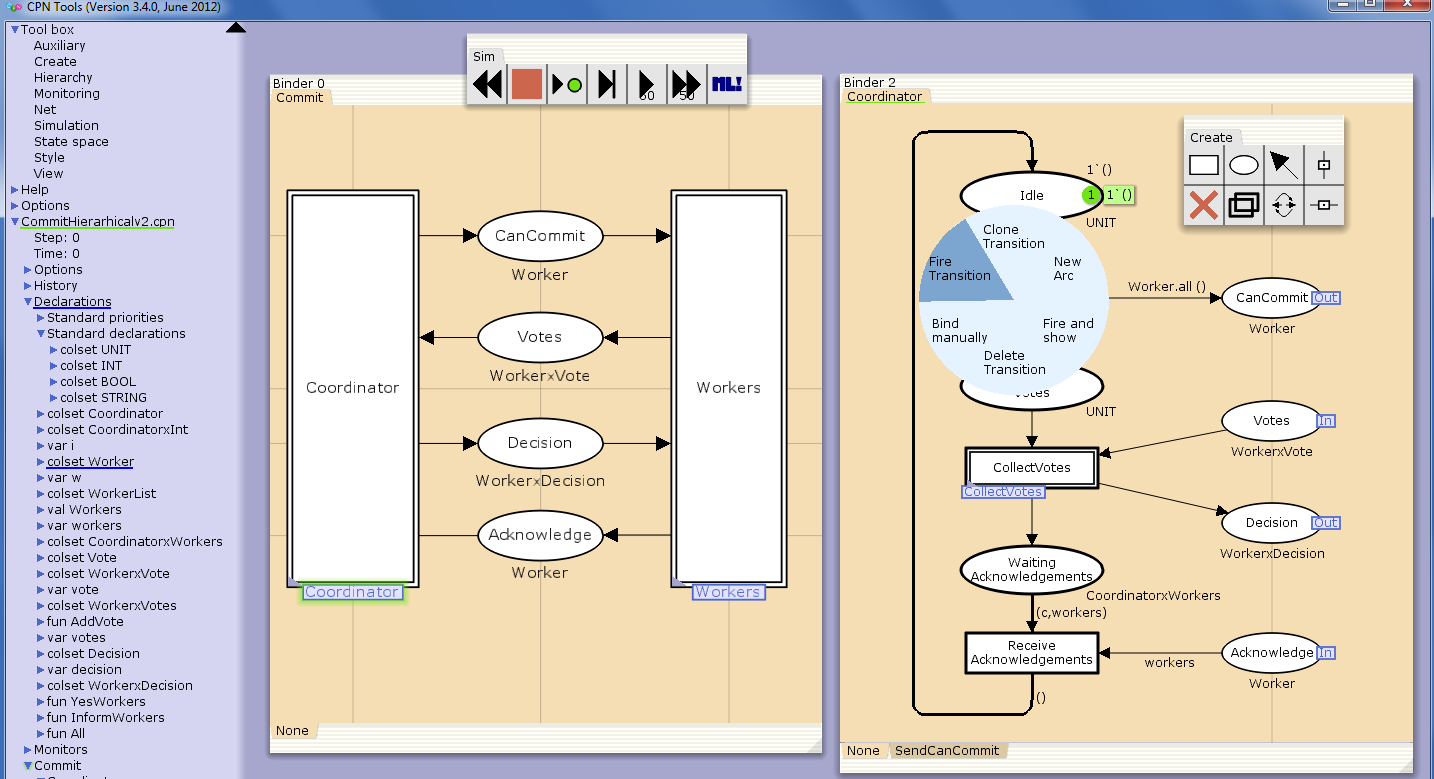
\includegraphics[scale=.37]{figures/cpntools.png}
\caption{The two-phase commit CPN model in CPN Tools}
\label{fig:cpntools}
\end{figure*}

Figure~\ref{fig:cpntools} provides a screen-shot of CPN Tools with the
CPN model considered in this paper. The user of CPN Tools works
directly with the graphical representation of the CPN model. The
graphical user interface of CPN Tools has no conventional menu bars
and pull-down menus, but is based on interaction techniques, such as
\concept{tool palettes} and \concept{marking menus}. The rectangular
area to the left is an \concept{index}. It includes the \figitem{Tool
  box}, which is available for the user to manipulate the declarations
and modules that constitute the CPN model. The \figitem{Tool box}
includes tools for creating, copying, and cloning the basic elements
of CPNs. It also contains a wide selection of tools to manipulate the
graphical layout and the appearance of the objects in the CPN
model. The latter set of tools is very important in order to be able
to create readable and graphically appealing CPN models. The remaining
part of the screen is the \concept{workspace}, which in this case
contains two \concept{binders} (the rectangular windows) and a
circular pop-up menu. Each binder may hold a number of items which can
be accessed by clicking the tabs at the top of the binder (only one
item is visible at a time). In the example shown, there are two
binders (with one item each). One binder (left) containing the
\figitem{Commit} module and one binder (right) containing the
\figitem{Coordinator} module. In addition, two tool palettes are
shown: one (\figitem{Sim}) containing the tools that can be used for
simulation of the model, and one tool palette (\figitem{Create})
containing the tools for creating CPN model elements. Items can be
dragged from the index to the binders, and from one binder to another
binder. A circular marking menu has been popped up on top of the right
binder. Marking menus are contextual menus that make it possible to
select among the operations possible on a given object. In the case of
Fig.~\ref{fig:cpntools}, the marking menu gives the operations that
can be performed on a transition.




\ignore{

 contains three
modules named \figitem{Protocol}, \figitem{Sender}, and
\figitem{Receiver}, while another binder contains a single module,
named \figitem{Network}, together with the declaration of the colour
set \smlcode{NOxDATA}. The two remaining binders contain four
different tool palettes to \figitem{Create} elements, change their
\figitem{Style}, perform \figitem{Simulations}, and construct
\figitem{State spaces}.

There are two kinds of binders. One kind contains the
elements of the CPN model, i.e., the modules and declarations. The
other kind contains the tools which the user applies to construct and
manipulate CPN models. The tools in a tool palette can be picked up
with the mouse cursor and applied. In the example shown, one binder
contains three modules named \figitem{Protocol}, \figitem{Sender}, and
\figitem{Receiver}, while another binder contains a single module,
named \figitem{Network}, together with the declaration of the color
set \smlcode{NOxDATA}. The two remaining binders contain four
different tool palettes to \figitem{Create} elements, change their
\figitem{Style}, perform \figitem{Simulations}, and construct
\figitem{State spaces}.
}

% syntax check and code generation and simulation

CPN Tools performs syntax and type checking, and contextual error
messages are provided to the user. The syntax check and code generation are
incremental and are performed in parallel with editing. This means
that it is possible to execute parts of a CPN model even if the model
is not complete, and that when parts of a CPN model are modified, a
syntax check and code generation are performed only on the elements
that depend on the parts that were modified. CPN Tools supports two
types of simulation: interactive and automatic. In an interactive
simulation, the user is in complete control and determines the
individual steps in the simulation, by selecting between the enabled
events in the current state. CPN Tools shows the effect of executing a
selected step in the graphical representation of the CPN model. In an
automatic simulation the user specifies the number of steps that are
to be executed and/or sets a number of stop criteria and
breakpoints. The simulator then automatically executes the model
without user interaction by making random choices between the enabled
events in the states encountered. Only the resulting state is shown in
the GUI but information about the executed steps can be collected in
various ways. CPN Tools also includes support for domain-specific
graphical feedback from simulations developed by Westergaard and
Lassen \cite{britney}.

In addition to the scientific work already cited, the following
persons significantly influenced the development of the computer
tools. Jawahar Malhotra got the idea to use the Standard ML language
as a basis for type definitions and net inscriptions in Design/CPN,
Ole Bach Andersen implemented the graphical interface of Design/CPN,
and S\o{}ren Christensen implemented the complex inference algorithms
for automatic binding of free variables during simulations. Hartmann
Genrich constributed to Design/CPN with knowledge and experience from
PrT nets. The graphical user interface of CPN Tools was designed
together with Michel Beaudouin-Lafon and Wendy McKay.

\ignore{
  The
simulator of CPN Tools exploits a number of advanced data structures
for efficient simulation of large hierarchical CPN models. The
simulator exploits the locality property of Petri nets to ensure that
the number of steps executed per second in a simulation is independent
of the size of the CPN model. This guarantees that simulation scales
to large CPN models.
}




